
%***************************************************************************
%
% CreditCruncher - A portfolio credit risk valorator
% Copyright (C) 2004 Gerard Torrent
%
% This program is free software; you can redistribute it and/or
% modify it under the terms of the GNU General Public License
% as published by the Free Software Foundation; either version 2
% of the License.
%
% This program is distributed in the hope that it will be useful,
% but WITHOUT ANY WARRANTY; without even the implied warranty of
% MERCHANTABILITY or FITNESS FOR A PARTICULAR PURPOSE.  See the
% GNU General Public License for more details.
%
% You should have received a copy of the GNU General Public License
% along with this program; if not, write to the Free Software
% Foundation, Inc., 59 Temple Place - Suite 330, Boston, MA 02111-1307, USA.
%
%
% implementation.tex - TeX documentation file
% --------------------------------------------------------------------------
%
% 2005/01/22 - Gerard Torrent [gerard@fobos.generacio.com]
%   . initial release
%
%***************************************************************************

\chapter{Implementaci\'on}
\label{sec:implementation}


\section{Interpretaci\'on del fichero de entrada}

El contenido esperado del fichero de entrada se encuentra
descrito en el documento \emph{CreditCruncher - Input File Reference}
que se adjunta junto al programa.
\newline
\newline
El fichero de entrada puede tener un tama\~no considerable. Por
este motivo la interpretaci\'on del fichero xml se realiza usando un
sistema orientado a eventos (tipo SAX). A continuaci\'on se
describen algunas de las validaciones mas importantes:

\paragraph{Formato.} Se verifica que se trata de un fichero XML
v\'alido que cumple la DTD. V\'ease \emph{W3C}\footnote{http://www.w3.org/XML/}
para m\'as informaci\'on relativa al formato XML.

\paragraph{Valores.} Cada valor tiene un tipo (int, long, double,
date, boolean o string), un rango de valores permitidos y un
indicador de obligatorio/opcional. Para cada valor se comprueba
que se cumplen los criterios descritos en
\emph{CreditCruncher - Input File Reference}.

\paragraph{Consistencia.} Cuando un valor se refiere a un identificador,
se comprueba que el objeto referenciado existe. Por ejemplo, cuando se
lee una transici\'on en la definici\'on de la matriz de transici\'on se
comprueba que los ratings han sido definidos anteriormente y que los
ratings referenciados existen.

\paragraph{Matriz de transici\'on.} Al leer la matriz de transici\'on
se verifica que cumple con las propiedades indicadas en
\ref{sec:mtransition:properties}.

\paragraph{Funci\'on de supervivencia.} En caso de estar definida
una funci\'on de supervivencia, se comprueba que se trata de una
funci\'on positiva mon\'otona decreciente que vale $1$ cuando $t=0$.

\paragraph{Matriz de correlaci\'on.} Se comprueba que se trata de
una matriz sim\'etrica (por comodidad, puede entrarse solamente
el triangulo superior, o inferior), con valores comprendidos
en $[-1,+1]$.

\paragraph{Criterios de parada.} Se comprueba que exista alg\'un
criterio de parada y que este sea realizable.

%---------------------------------------------------------------------------

\section{Particionamiento del tiempo}

Para realizar el particionamiento del tiempo se necesita la fecha inicial, $t_0$,
la longitud (en meses naturales) de cada intervalo, $StepLength$, y el n\'umero
de pasos a considerar, $NumSteps$. Las fechas de la partici\'on son:
\begin{displaymath}
t_i = t_0 + i \cdot StepLength \qquad i \in \{0, 1, 2, \cdots, NumSteps\}
\end{displaymath}

Entendemos que a\~nadir $n$ meses a una fecha consiste en incrementar el
mes de la fecha inicial en $n$ meses, realizando un incremento de a\~no si
es preciso. Si el d\'ia de mes de la fecha inicial no existe en el mes de
la fecha final, consideramos como d\'ia de la fecha final el m\'aximo d\'ia
del mes de la fecha final, en caso contrario, el mismo d\'ia de mes de la
fecha inicial.
\newline
\newline
Supongamos que $t_0=30/10/2004$, $StepLength=2$ y $NumSteps=6$, entonces la
partici\'on del tiempo es: $30/10/2004$, $30/12/2004$, $28/02/2005$, $30/04/2005$,
$30/06/2005$, $30/08/2005$ y $30/10/2005$. Obs\'ervese como el d\'ia del mes de
Febrero es el $28$ por no existir los d\'ias $29$ y $30$ de dicho mes.

\begin{figure}[!hb]
\begin{center}
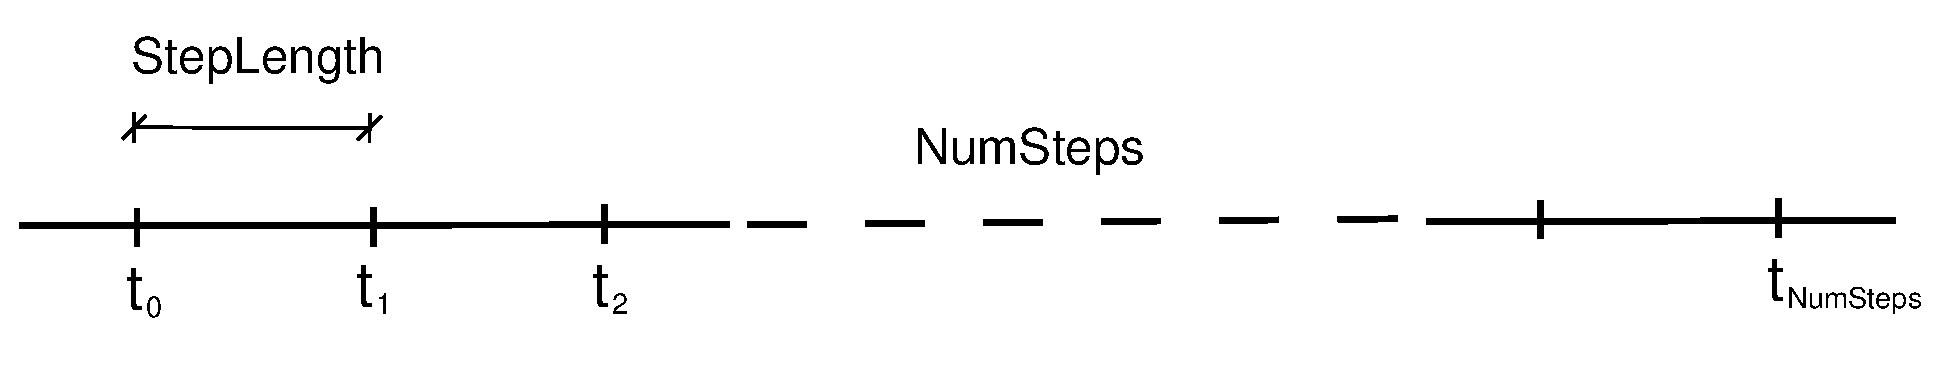
\includegraphics[width=10cm,angle=0]{./images/time.eps}
\caption{Particionamiento del tiempo}
\label{timetranches}
\end{center}
\end{figure}

%---------------------------------------------------------------------------

\section{Mapeo del cashflow}

Sea $t_0, t_1, t_2, \cdots, t_k$ la partici\'on de tiempo usada.
Dado un cashflow $(t_v,V)$ lo mapeamos en la estructura
temporal de la siguiente forma:

\begin{enumerate}
\item Si $t_v < t_0$, entonces $(t_v,V) \longrightarrow (t_0,0)$
\item Si $t_{i-1} < t_v \leq t_i$, entonces $(t_v,V) \longrightarrow (t_i,V \cdot \Upsilon(t_v,t_i))$
\item Si $t_k < t_v$, entonces $(t_v,V) \longrightarrow (t_k,0)$
\end{enumerate}

donde $\Upsilon(t_v,t_i)$ es el coeficiente de transporte entre $t_v$ y $t_i$.

\begin{figure}[!hb]
\begin{center}
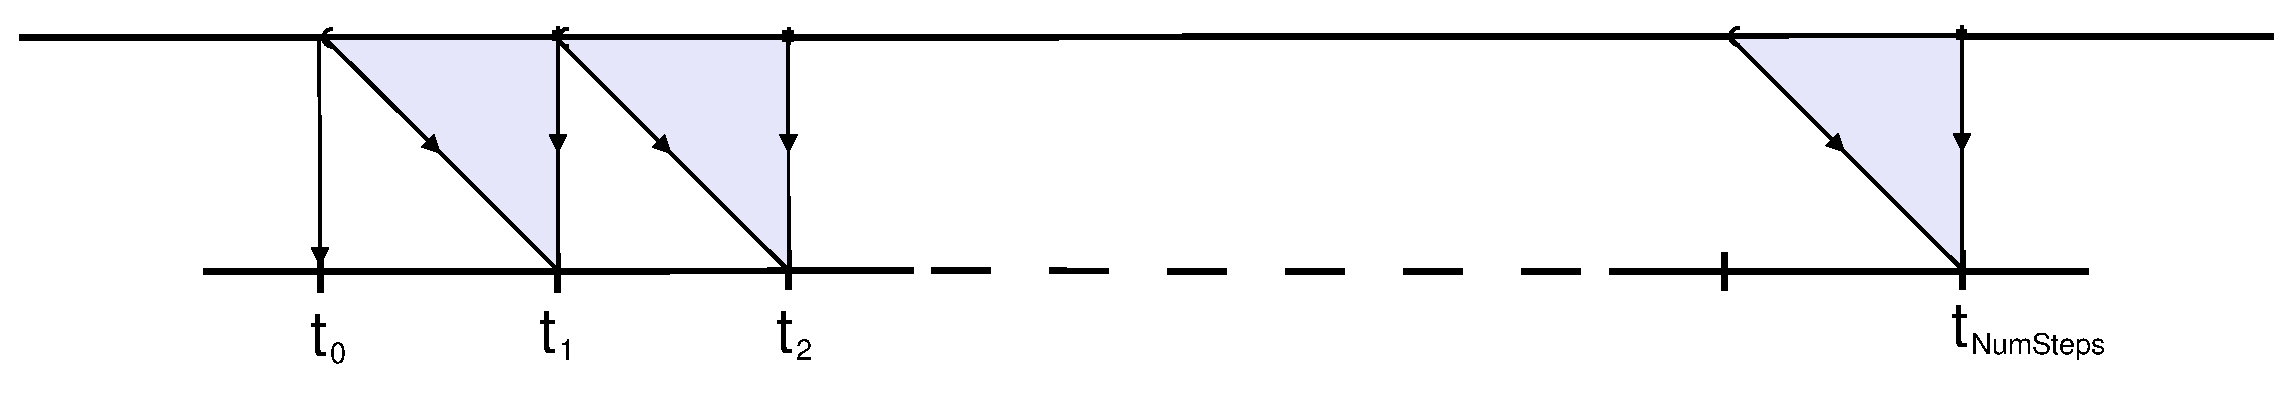
\includegraphics[width=10cm,angle=0]{./images/cashflowmapping.eps}
\caption{CashFlow mapping}
\label{timetranches}
\end{center}
\end{figure}

Veamos un ejemplo. Consideramos $\Upsilon(t_i,t_j)=1$ para no complicar los c\'alculos.
A la izquierda se representa el cashflow original (sin estar mapeado a los nodos de
tiempo). A la derecha se encuentra el mismo cashflow mapeado a los nodos de tiempo.
\newline
\newline
\begin{minipage}[c]{0.5\columnwidth}%
\centering
\begin{tabular}{c|r}
\textbf{Date} & \textbf{Cashflow} \\
\hline
17/04/2004 & -10.00 \\
           &        \\
           &        \\
05/01/2005 &   1.00 \\
20/01/2005 &   2.00 \\
           &        \\
15/03/2005 &   3.00 \\
           &        \\
           &        \\
30/08/2005 &   4.00 \\
           &        \\
15/12/2005 &   5.00 \\
\end{tabular}
\end{minipage}%
\begin{minipage}[c]{0.5\columnwidth}%
\centering
\begin{tabular}{c|c|c}
\textbf{$t_i$} & \textbf{Date}  & \textbf{Cashflow} \\
\hline
      &            &      \\
$t_0$ & 30/10/2004 & 0.00 \\
$t_1$ & 30/12/2004 & 0.00 \\
      &            &      \\
      &            &      \\
$t_2$ & 28/02/2005 & 1.00 + 2.00 \\
      &            &      \\
$t_3$ & 30/04/2005 & 3.00 \\
$t_4$ & 30/06/2005 & 0.00 \\
$t_5$ & 30/08/2005 & 4.00 \\
$t_6$ & 30/10/2005 & 0.00 \\
      &            &      \\
\end{tabular}
\end{minipage}%

%---------------------------------------------------------------------------

\section{Mapeo del netting}

Sea $t_0, t_1, t_2, \cdots, t_k$ la partici\'on de tiempo usada.
Calculamos el netting en un nodo, $t_i$, de la partici\'on de la
siguiente forma:

\begin{enumerate}
\item Si existe un netting anterior, $(t_a,W_a)$, y otro posterior, $(t_b,W_b)$,
a $t_i$, entonces el valor del netting en $t_i$ es
$A + (B-A) \cdot \frac{t_i-t_a}{t_b-t_a}$ donde
$A=\Upsilon(t_a,t_i) \cdot W_a$ y $B=\Upsilon(t_b,t_i) \cdot W_b$.
\item Si no existe un netting anterior a $t_i$ entonces el valor del netting
en $t_i$ es $0$.
\item Si existe un netting entre $t_{i-1}$ y $t_i$, $(t_a,W_a)$, pero no existe un
netting posterior a $t_i$, entonces el valor del netting en $t_i$ es
$\frac{t_a-t_{i-1}}{t_i-t_{i-1}} \cdot W_a \cdot \Upsilon(t_a,t_i)$
\end{enumerate}

\begin{figure}[!hb]
\begin{center}
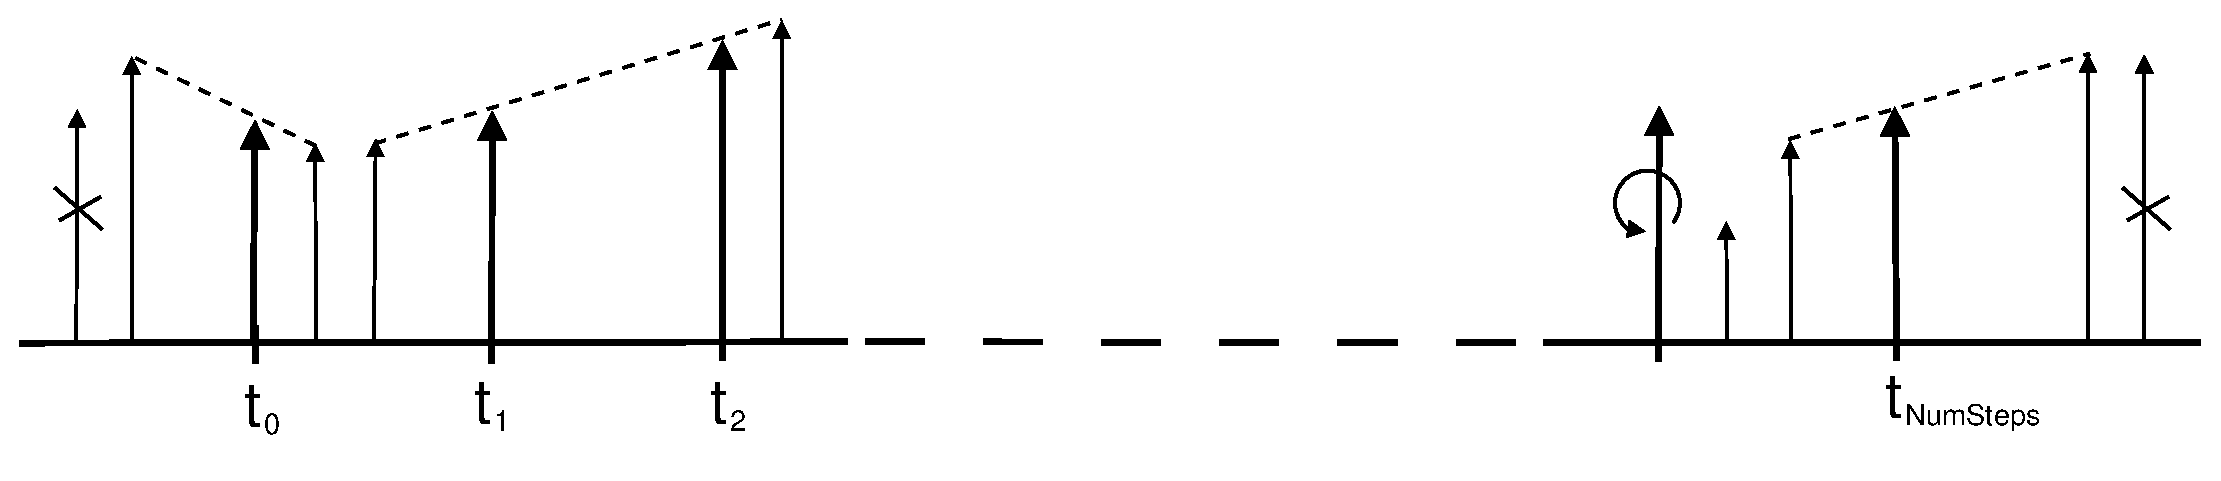
\includegraphics[width=10cm,angle=0]{./images/nettingmapping.eps}
\caption{Netting mapping}
\label{timetranches}
\end{center}
\end{figure}

%---------------------------------------------------------------------------

\section{Inicializaci\'on del problema}


\begin{figure}[!hb]
\begin{center}
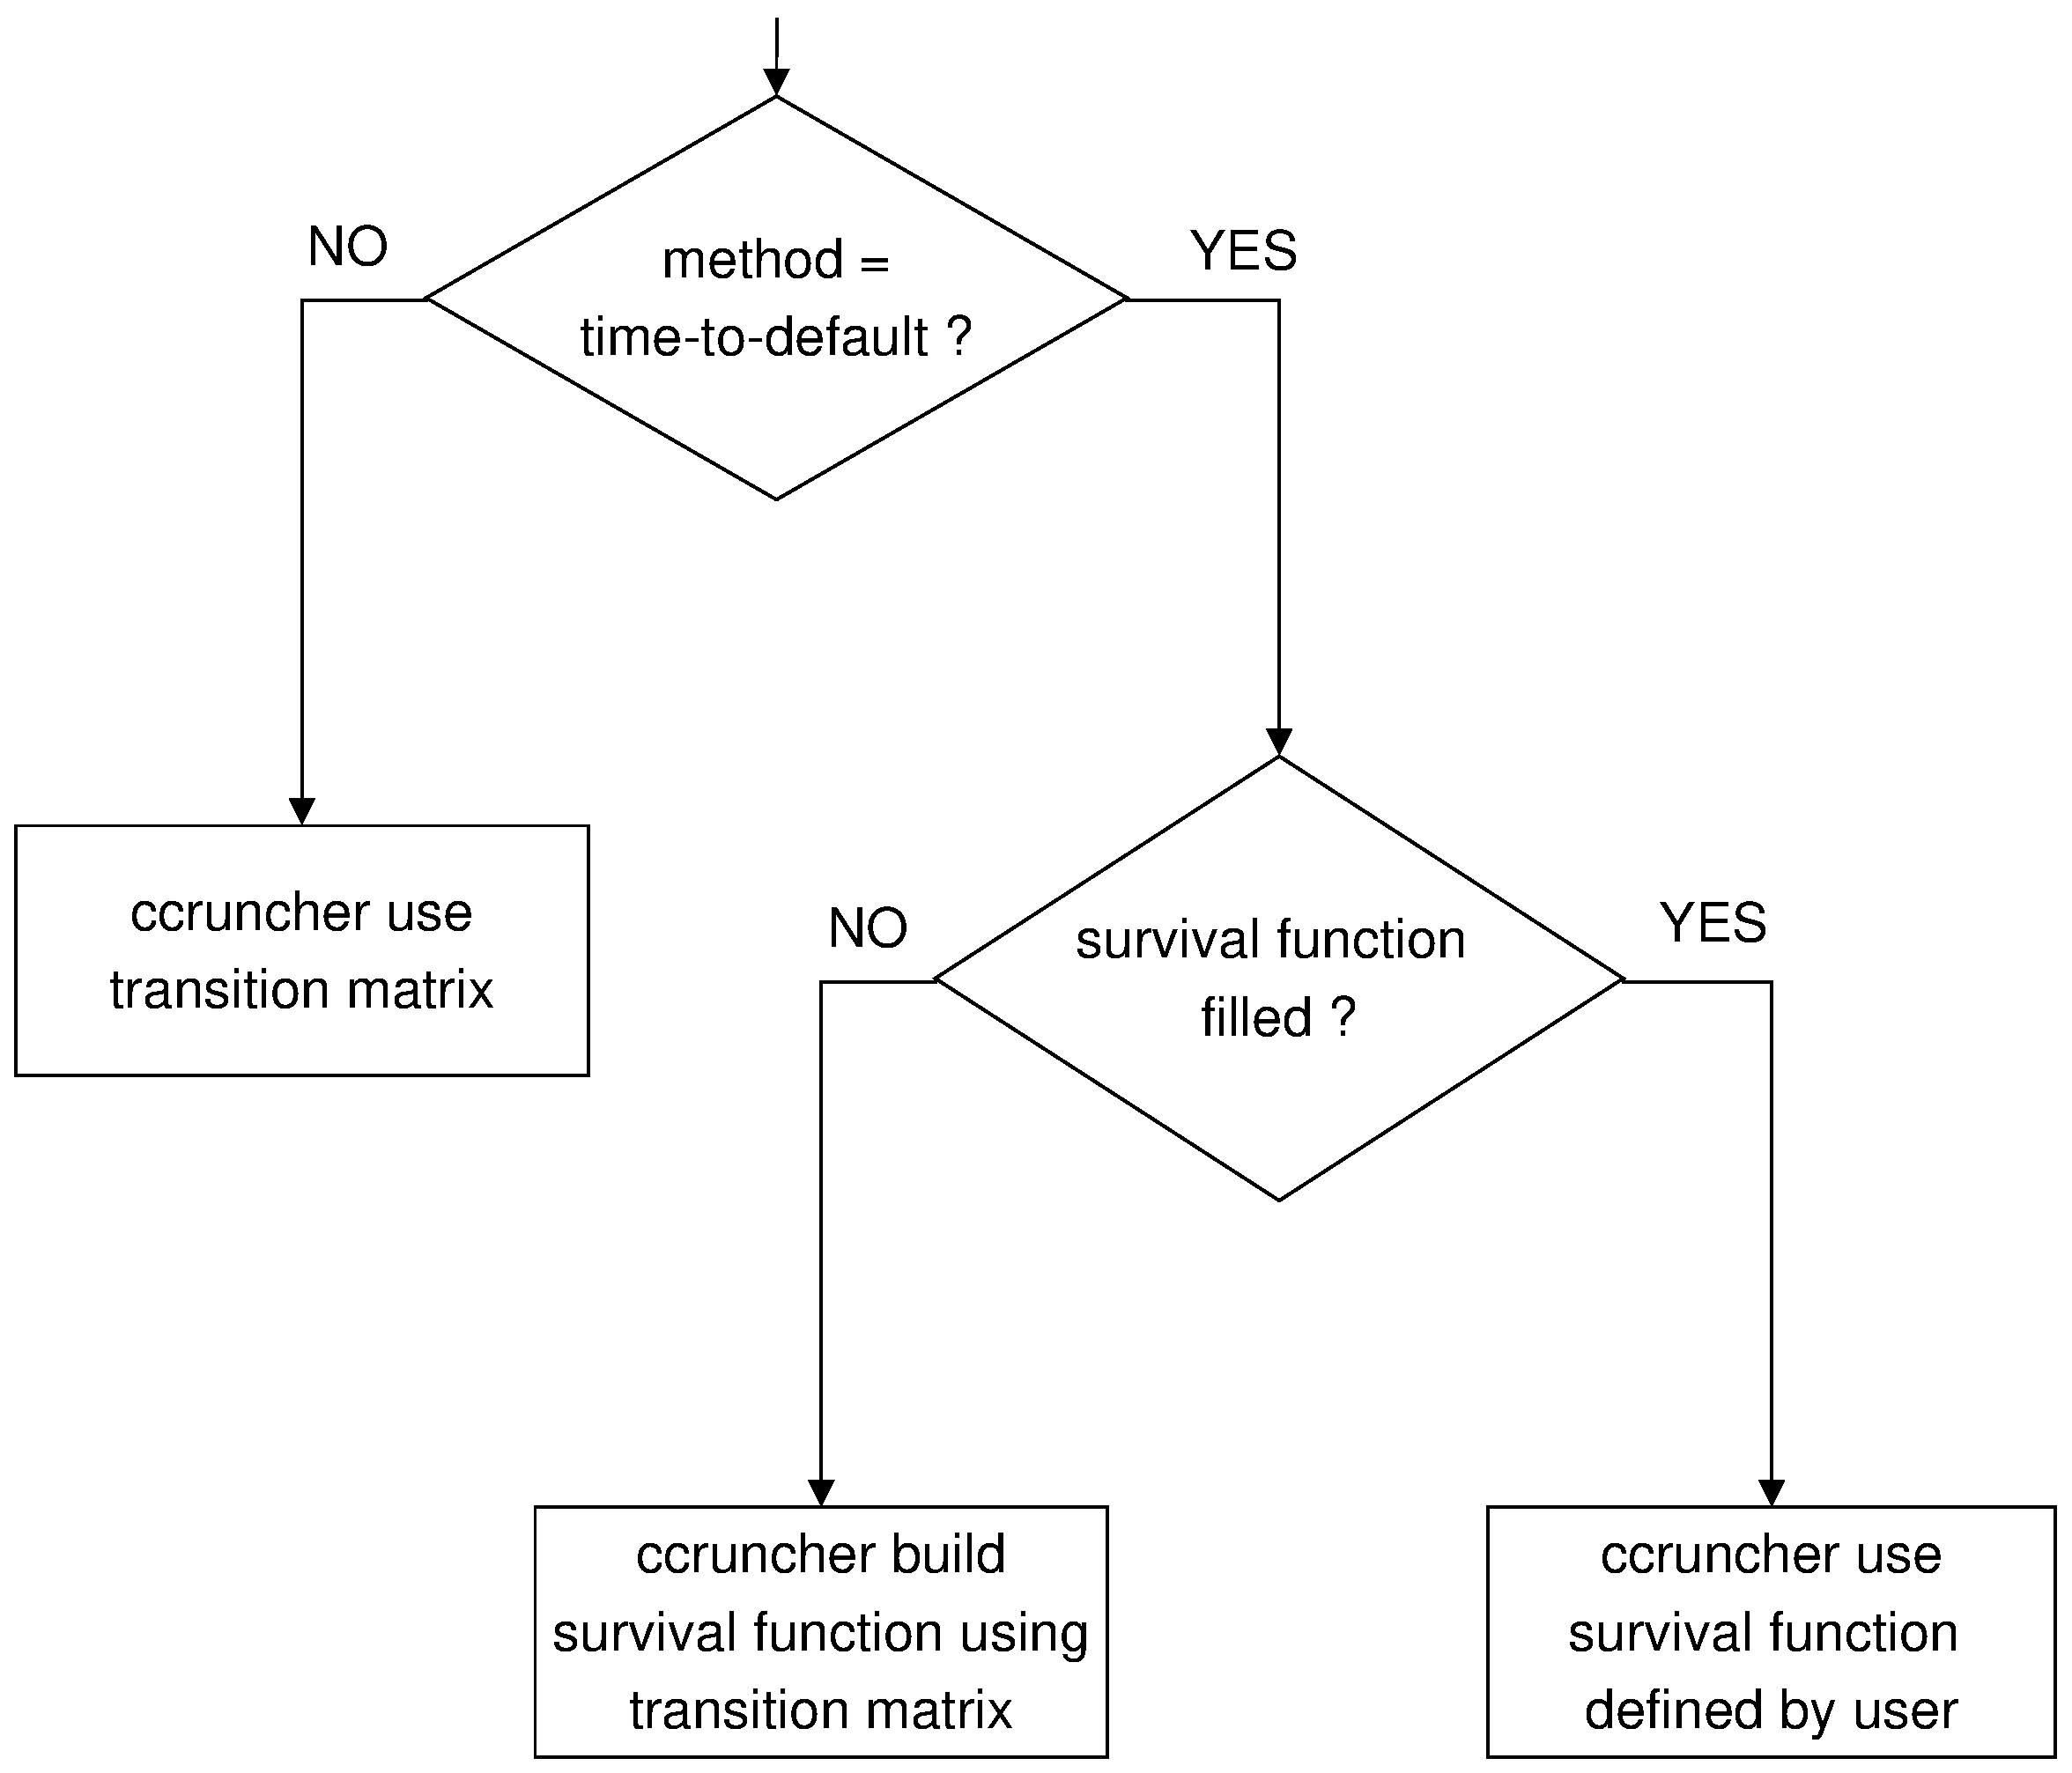
\includegraphics[width=10cm,angle=0]{./images/decisiontree1.eps}
\caption{Decisi\'on en funci\'on del m\'etodo}
\label{decisiontree1}
\end{center}
\end{figure}

precalculo de los valores en los nodos


\section{Proceso de agregaci\'on}

TODO: descripcion de los agregadores y metodo usado para evitar recalculo 
de los activos en cada simulacion + Agregaci\'on de productos


\section{Dimensiones del problema}

TODO: Estimaciones de uso de memoria, estimaci\'on del numero de operaciones,
estimacion del tiempo de computo


\section{Convergencia de la soluci\'on}

TODO: N\'umero de iteraciones necesarias, aceleraci\'on de la convergencia
usando metodolog\'ia antithetic

convergencia media, varianza, var (estimadores, graficos, etc.)
